\documentclass[11pt]{article}
\usepackage[utf8]{inputenc}
\usepackage[czech]{babel}
\usepackage[utf8]{inputenc}
\usepackage{times}
\usepackage{graphicx}
\usepackage[a4paper,top=30mm,left=20mm,textwidth=17cm,textheight=24cm]{geometry}

\begin{document}

    \begin{titlepage}
        \begin{center}
            
\includegraphics[width=1\linewidth]{fit logo.png} \\
            
            \vspace{\stretch{0.382}}
            
            \Huge{Dokumentace projektu IFJ} \\ 
            \LARGE{Implementace překladače imperativního jazyka IFJ21} \\
            \Large{Tým 027, varianta 1} \\
            \Large{[BOOLTHEN, FUNEXP, OPERATORS]}
            
            \vspace{\stretch{0.618}}
        \end{center}
        \hfill
        \begin{center}
        \LARGE
            \begin{tabular}{l  l  l}
                \textbf{Vojtěch Dvořák} & \textbf{xdvora3o} & \; xx\% \\
                 Tomáš Dvořák & xdvora3r & \; xx\% \\
                 Juraj Dedič &  xdedic07 & \; xx\% \\
                 Radek Marek & xmarek77 & \; xx\%
            \end{tabular}
        \end{center}
    \end{titlepage}
    
    \setcounter{page}{1}
    \tableofcontents
    \clearpage
    
    \section{Úvod}
        Cílem projektu bylo vytvořit překladač v jazyce C, který zpracuje kód ze zdrojového jazyka IFJ21 (podmnožinou jazyka Teal) a následně jej přeloží do cílového jazyka IFJcode21. \\
    	\indent Program načte vstup ze standartního vstupu, zanalyzuje a v případě, že načtený kód neobsahuje žádné chyby, vygeneruje výsledný kód. V opačném případě ukončí provádění a vrátí chybový kód odpovídající typu chyby.
	
	\section{Implementace}
	
	\subsection{Lexikální analýza}
    	Náš lexikální analyzátor je řízen konečným automatem, který je implementován pomocí tabulky přechodových funkcí (staticky alokované pole). Stavy konečného automatu jsou identifikovány k tomu určeným výčtovým datovým a tyto identifikátory zároveň představují index zmíněné tabulky. \\
    	\indent Přechodovými funkcemi označujeme funkce, které obsahují množství podmínek, na základě, kterých se rozhoduje, do kterého stavu se automat přepne, případně zda má analyzátor vrátit token s příslušných typem. \\
     	\indent Token v našem analyzátoru vyznačuje strukturu obsahující typ, atribut a index, který ukazuje na  určité místo v bufferu, v němž jsou uloženy hodnoty všech tokenů, vyjma těch předdefinovaných (klíčová slova, oddělovače, operátory). Ty jsou uloženy ve speciálních statických polích kvůli lepšímu hospodaření s alokovanou pamětí. Pokud během lexikální analýzy dojde k chybě, automat vrátí token s chybovým typem. 

	\subsection{syntaktická analýza}
	
	\subsection{Sémantická analýza}
    	Souběžně se syntaktickou analýzou probíhá sémantická analýza. Ke kontrole se používá zejména tabulka symbolu společně s návratovými hodnotami precedenčního syntaktického analyzátoru. Při kontrole datových typů ve zdrojovém kódu (jazyce) používáme speciální výčtový datový typ a znaky uložené v dynamicky alokovaných řetězcích, které identifikují datové typy a jejich počet. Toto nám umožňuje snadno provádět tyto typové kontroly pří mnohonásobném přiřazení, nebo funkcí s více než jednou návratovou hodnotou. \\
    	\indent V případě aritmetických, řetězcových a relačních výrazů	 analyzátor kontroluje typovou kompatibilitu na základě staticky alokované tabulky, ve které se nachází popis možných datových typů pro zpracovávanou operaci. Při redukci, je výsledný typ operace propagován do struktury vzniklého neterminálu.

	\subsection{Generování kódu}
	
    \section{Datové struktury}
    
    \subsection{Binární vyhledávací strom}
        Tuto strukturu využíváme, jak nám ukládá zadání, pro implementaci tabulky symbolů. Kromě základní struktury a operací jsme implementovali možnost zřetězit více BVS. Zřetězení jsme dosáhli využitím přítomností indexů nadřazeného bloku, který je uložen v dynamickém poli. Toho využíváme při hledání proměnných v nadřazených blocích kódu.\\
        Při iplementaci jsme vycházeli z našich řešení projektů do předmětu IAL.
    
    \subsection{Dynamické pole}
        Vyjma sttaticky alokovaných polí, využity například pro snadnou implementaci precedenční tabulky, tabulky vestavěných funkci nebo tabulku klíčových slov, náš překladač také využívá dynamicky alokovaná pole. \\
        \indent Rozhodli jsmme se pro tuto možnost hlavně z důvodů teoreticky neomezené kapacity a spojitého uložení dat v paměti, lze tak jednoduše vypisovat v nich uložené řetězce pomocí standartních funkcí. Náročné realokace při zvětšování nejsou tak podstatné, protože náš systém není real-time aplikací.
    
    \subsection{Zásobník}
        Zásobník hraje naprosto zásadní roli v precedenčním syntaktickém analyzátoru při zpracování veškerých výrazu. Struktura se však osvědčila i v jiných částech našeho překladače. \\
        \indent Příkladem je vyhodnocování mnohonásobných přiřazovacích operací, kde se jednotlivé prvky přiřazují směrem z prava do leva. V tomto případě jsou do zásobníku ukládány ukazatele na sekvence instrukcí v cílovém jazyce, které jednotlivé výrazy reprezentují. Následně se zásovník vyprázdňuje jsou napojovány na hlavní tělo generovaného programu. \\
        \indent Náš zásobník je implementován prostřednictvím dynamicky alokoveného pole, umožnuje realokaci a následné zvětšení kapacity v případě potřeby. Pro snadnější a čístší implementaci jsme si zavedli makro, které dokáže snadno vygenerovat tuto strukturu pro různé datové typy, což výrazně snižuje redundanci kódu.
        
    \subsection{Dvojsměrně vázaný seznam}
        Strukturu využíváme pro uložení instrukcí cílového jazyka před jejich vypsáním na standartní výstup. Každá položka obsahuje dynamický řetězec s zpravidla jednou instrukcí a odkazy na předchozí a následující instrukci. Tato reprezentace umožňuje cílový kód takřka libovolně editovat v průběhu překladu, tato vlastnost je důležitý zejména při deklarací proměnných hodnot uvnitř těla cyklu. \\
        \indent Díky dvojsměrně vázanému seznamu si můžeme uchovávat ukazaten před začátkem cyklu, kam postupně vkládáme deklarace v cílovém jazyce, ty by uvniř cyklu mohly způsopbit chybu z důvodů redeklarace proměnných.
        
    
    \section{Práce v týmu}
    
    \subsection{Rozdělení práce}
    
    \subsection{Verzovací systém}
        Jako verzovací systém jsme si vybrali Git a vzdálený repozitář na serveru GitHub. \\
    	\indent Tento výběr nám dovolil pracovat zároveň na více částech programu najednou. Každý člen teamu pracoval ve vlastním odvětví a při určitých intervalech se všechna naše řešení spojili do jednoho. 

    \subsection{Komunikace}
        Komunikace probíhala z převážně přes Discord, kde jsme využívaly textové a hlasové místnosti a připínání důležitých věcí a událostí. \\
    	\indent Pravidelně jsme se scházeli jednou týdne, ale s blížícím datem odevzdání se počet setkání zvyšoval.

    \section{Diagram konečného automatu}
        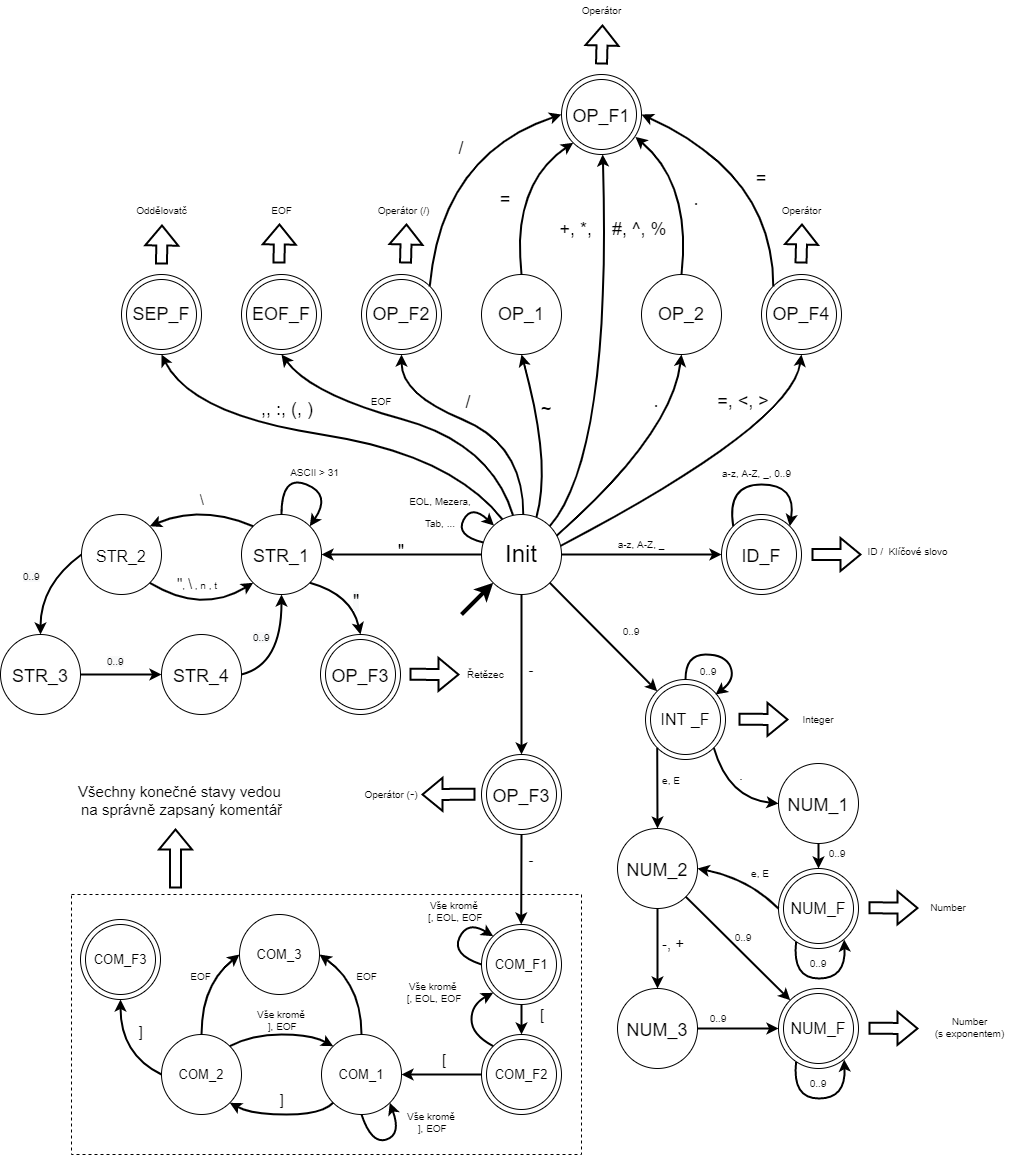
\includegraphics[width=1\linewidth]{FSM.png}
        \pagebreak
    
    \section{LL -- Gramatika}
        \verb|<program> -> <prolog> <global-statement-list>| \\
        \verb|<prolog> -> require "ifj21"| \\
        \verb|<statement-list> -> <statement> <statement-list>| \\
        \verb|<statement-list> -> [eps]| \\
        \verb|<statement-list> -> <function-call>| \\
        \verb|<global-statement> -> global [id] : function(<param-list>) <type-list>| \\
        \verb|<statement> -> local  [id] : [type] <value-assignment>| \\
        \verb|<value-assignment> -> [eps]| \\
        \verb|<value-assignment> -> = <expression>| \\
        \verb|<statement> -> <assignment>| \\
        \verb|<assignment> -> <id-list> = <expression-list>| \\
        \verb|<id-list> -> [id] <id-list-1>| \\
        \verb|<id-list-1> -> , [id] <id-list-1>| \\
        \verb|<id-list-1> -> [eps]| \\
        \verb|<multiple-assignment> -> , [id] <multiple-assignment> <expression> , -->| \\
        \verb|<statement> -> if <expression> then <statement-list> <else-branch> end| \\
        \verb|<else-branch> -> [eps]| \\
        \verb|<else-branch> -> else <statement-list>| \\
        \verb|<statement> -> while <expression> do <statement-list> end| \\
        \verb|<while>| \\
        \verb|<global-statement> -> <function-call>| \\
        \verb|<statement> -> [function-id](<argument-list>)| \\
        \verb|<argument-list> -> <argument> <argument-list-1>|  \\
        \verb|<argument-list> -> [eps]|  \\
        \verb|<argument-list-1> -> , <argument> <argument-list-1>| \\
        \verb|<argument-list-1> -> [eps]| \\
        \verb|<argument> -> <expression>| \\
        \verb|<global-statement-list> -> <global-statement> <global-statement-list>| \\
        \verb|<global-statement> -> function [id](<param-list>)<type-list> <statement-list> end| \\
        \verb|<function-type-def> -> [eps]| \\
        \verb|<function-type-def> -> <type-list>| \\
        \verb|<param-list> -> [id] : [type] <param-list-1>| \\\,
        \verb|<param-list-1> -> , [id] : [type] <param-list-1>| \\
        \verb|<param-list-1> -> eps| \\
        \verb|<type-list> -> [eps]| \\
        \verb|<type-list> -> : [type] <type-list-1>| \\
        \verb|<type-list-1> -> , [type] <type-list-1>| \\
        \verb|<type-list-1> -> [eps]| \\
        \verb|<statement> -> return <expression-list>| \\
        \verb|<statement> -> return| \\
        \verb|<expression-list> -> <expression> <expression-list-1>| \\
        \verb|<expression-list-1> -> , <expression> <expression-list-1>| \\
        \verb|<expression-list-1> -> [eps]| \\

        \pagebreak
        
    \section{LL -- Tabulka}
        
    \section{Precedenční tabulka}
        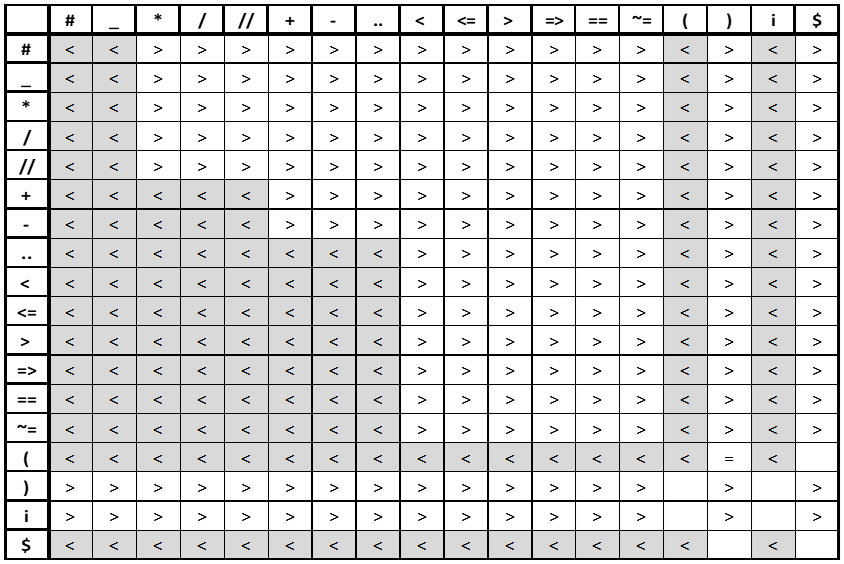
\includegraphics[width=1\linewidth]{precedenční tabulka.png}
        \pagebreak    
\end{document}
